% ICRC-2021 
%
% Deadline 5 July
% Maximum 8 pages

% Please make sure you insert your
% data according to the instructions in PoSauthmanual.pdf
\documentclass[a4paper,11pt]{article}
\usepackage{pos} 

\usepackage[utf8]{inputenc} % Включаем поддержку UTF8
\usepackage[T2A]{fontenc}
\usepackage[english]{babel}   % убрать русский перед отправкой статьи % влияет на язык подписей к рисункам и таблицам
\usepackage[modulo]{lineno}
\usepackage{graphicx}
\graphicspath{{figures/}}
%\usepackage[pdftex, backref, colorlinks]{hyperref}
\usepackage{booktabs}
\usepackage{todonotes}
\usepackage{caption}
\usepackage{subcaption}
%http://ctan.math.washington.edu/tex-archive/macros/latex/contrib/easy-todo/easy-todo.pdf
%\usepackage[enable]{easy-todo}

\title{A drone-borne installation for studying the composition of cosmic rays in the range of 1--1000~PeV by registering the reflected Cherenkov light of EAS}
\ShortTitle{SPHERE-3 project} 

%\date{June 2021}
\author*[a,b]{I. A. Vaiman}
\author[b]{D. V. Chernov}
\author[b]{E. A. Bonvech}
\author[c,d]{M. Finger}
\author[c,d]{M. Finger Jr}
\author[a,b]{V. I. Galkin}
\author[a]{V. A. Ivanov}
\author[a]{V. S. Latypova}
\author[a,b]{D. A. Podgrudkov}
\author[b]{T. M. Roganova}

\affiliation[a]{Faculty of physics, Lomonosov Moscow State University,\\Lininskie gory, 1, Moscow, Russia}
\affiliation[b]{Skobeltsyn Institute for Nuclear Physics Lomonosov Moscow State University,\\Lininskie gory, 1, Moscow, Russia}
\affiliation[c]{Faculty of Mathematics and Physics, Charles University,\\18000 Prague, Czech Republic}
\affiliation[d]{Joint Institute for Nuclear Research,\\Dubna, Russian Federation}

\emailAdd{gosha.vaiman@gmail.com}
%\emailAdd{chr@dec1.sinp.msu.ru}
%\emailAdd{bonvech@yandex.ru}
%\emailAdd{michael.finger@cern.ch}
%\emailAdd{miroslav.finger@cern.ch}
%\emailAdd{v\_i\_galkin@mail.ru}
%\emailAdd{ivanov.va18@physics.msu.ru}
%\emailAdd{2000vi0501g@mail.ru}
%\emailAdd{d.a.podgrudkov@physics.msu.ru}
%\emailAdd{rogatm@yandex.ru}

\abstract{
Current technical design of the SPHERE project’s new detector is presented. The SPHERE project is aimed at primary cosmic ray studies in the 1--1000 PeV energy range using reflected Cherenkov light. The concept of a drone-mounted detector with a photosensitive camera based on silicon photomultipliers is discussed. The combination of the reflected CL registration method with specific data analysis approaches is a unique feature of this project. The developed earlier event-by-event data analysis approach allows to carry out primary particle mass reconstruction and primary cosmic ray mass composition studies with high accuracy. This is achieved through careful analysis of each EAS Cherenkov light lateral distribution function without building any kind of intermediate distributions of any `typical' characteristics.
}

\FullConference{37$^{\rm{th}}$ International Cosmic Ray Conference (ICRC 2021)\\
		July 12th -- 23rd, 2021\\
		Online -- Berlin, Germany} 

%\keywords{EAS, Cherenkov light, detector, proposal}


\begin{document}

\newcommand{\todoi}[1]{\todo[inline]{ #1}}
% \renewcommand{\@makefnmark}{\hbox{\@textsuperscript{\normalfont\@thefnmark}}}
% \def\@makefnmark{\hbox{\@textsuperscript{\normalfont\@thefnmark}}}

\maketitle

\section{Introduction}

%Vavilov-Cherenkov radiation (or Chereknov light, CL) produced by charge particles of an extensive air shower (EAS) in atmosphere was theoretically predicted by P.M.S.~Blackett in late 1940s~\cite{Blackett1948} and first detected in early 1950s by W.~Galbraith and J.V.~Jelley~\cite{Galbraith1953} and by N.M.~Nesterova and A.E.~Chudakov~\cite{Nesterova1955}. Chudakov, who's centenary is celebrated this year, then developed the cosmic ray (CR) studies technique based on detection of Cherenkov light from EAS in late 1950s~\cite{Chudakov1958,ICRC1960} which few years later became the beginnings of the gamma-astronomy~\cite{Chudakov1962}.

Vavilov-Cherenkov radiation (or Chereknov light, CL) produced by charge particles of an extensive air shower (EAS) in atmosphere was theoretically predicted in late 1940s and first detected in early 1950s. A.E. Chudakov, who's centenary is celebrated this year, then developed the cosmic ray (CR) studies technique based on detection of Cherenkov light from EAS in late 1950s~\cite{ICRC1960} which few years later became the beginnings of the gamma-astronomy.%~\cite{Chudakov1962}.

After A.E. Chudakov's and G.T. Zatsepin's works direct CL became known as an important EAS registration channel. In particular, CL lateral distribution is indicative of the shower development details and can be used to infer both the energy and the mass of the primary particle.%~\cite[e.g.][]{Budnev2013,Knurenko2013}.

In 1974 A.E. Chudakov proposed a new experimental technique for CR studies --- detection of the reflected CL from EAS using electro-optical converters~\cite{chu74:VKKL74}. Reflected EAS CL technique was adopted and improved by R.A. Antonov who proposed the use of Schmidt optical scheme with a PMT-based camera. Later this approach transformed into the SPHERE project (see overview in~\cite{Ant15a}). SPHERE-1 detector performed measurements in 1997--2000 and SPHERE-2 detector performed measurements in 2011--2013. A new detector in the SPHERE project is now in development stage and is described below.

\subsection{Reflected Cherenkov light}

EAS CL light is observed by a detector from a certain altitude after it is first reflected from the `screen'. The schematic view of the technique is given in Fig.~\ref{fig:DirectCL}. In previous SPHERE implementations and the snow-covered ice of Lake Baikal played the role of such `screen'. Snow has a high overall albedo (up to 95\%) and an almost isotropic bidirectional reflectance distribution~\cite{Warren1982} --- crucial qualities for this method.

\begin{figure}
\centering
    \begin{minipage}{.3\textwidth}
        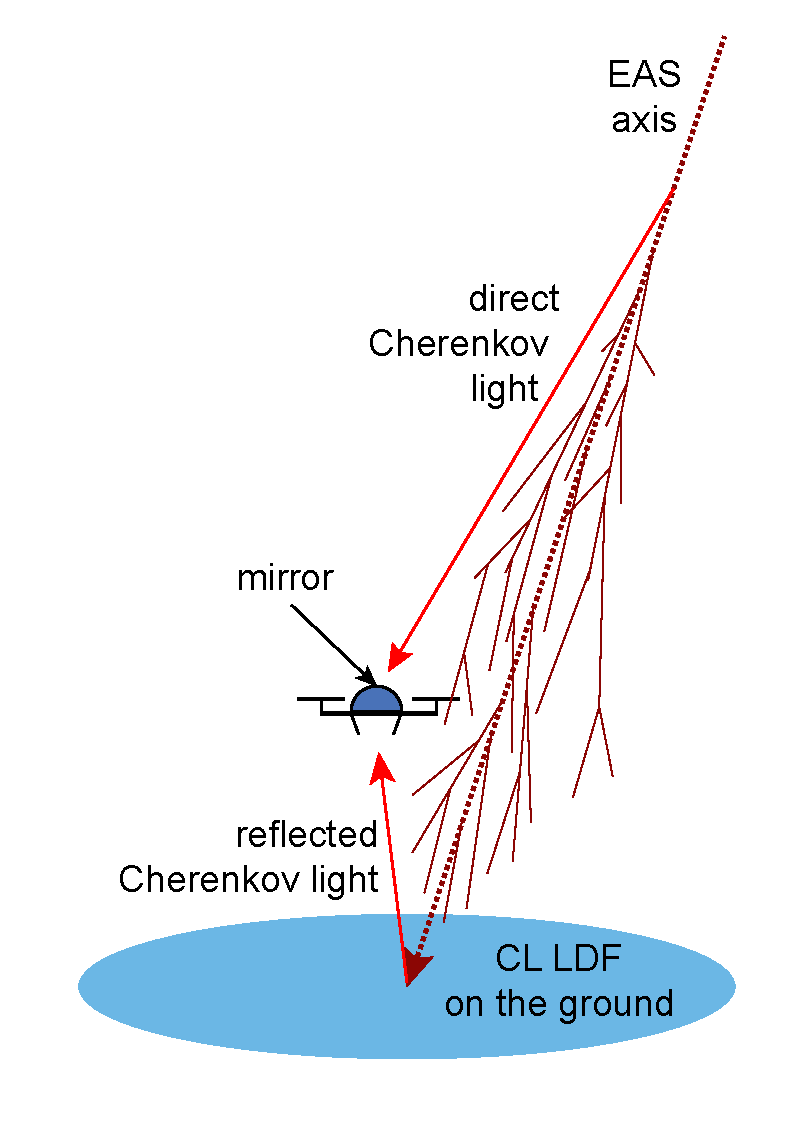
\includegraphics[width=1\textwidth]{DirectCL.pdf}
        \caption{Overview of the proposed SPHERE-3 detector operation with both reflected and direct CL being observed.}
        \label{fig:DirectCL}
        \end{minipage}
    \hfill
    \begin{minipage}{.67\textwidth}
        \centering
        \begin{subfigure}[t]{0.42\textwidth}
            \centering
            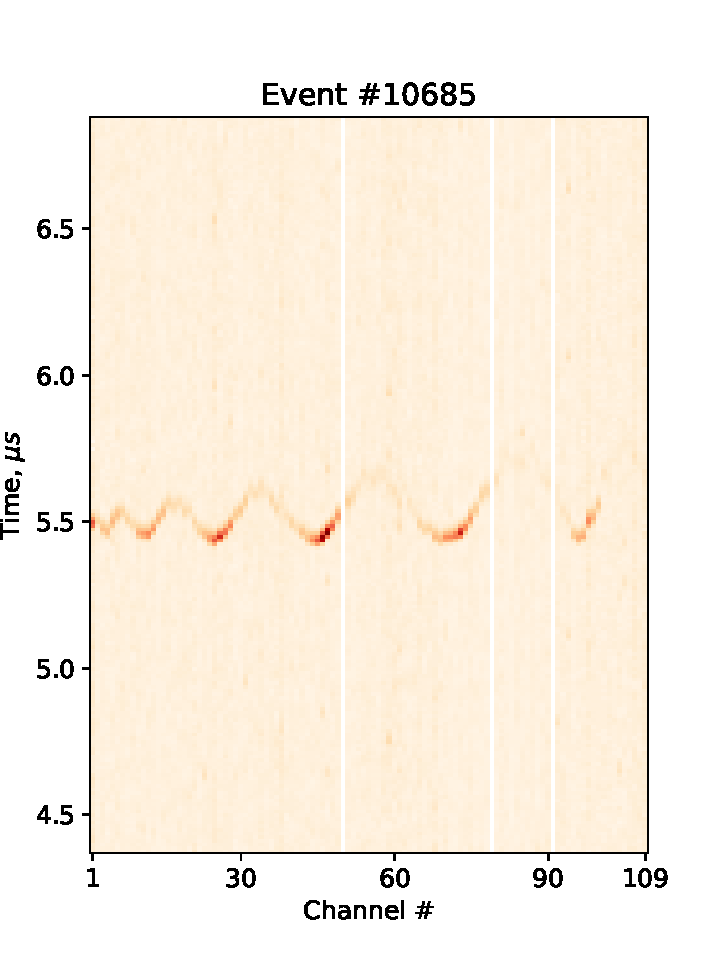
\includegraphics[width=\textwidth]{reflected-event}
            \caption{Reflected CL event}
            \label{fig:reflected-ev-1}
        \end{subfigure}
        \begin{subfigure}[t]{0.42\textwidth}
            \centering
            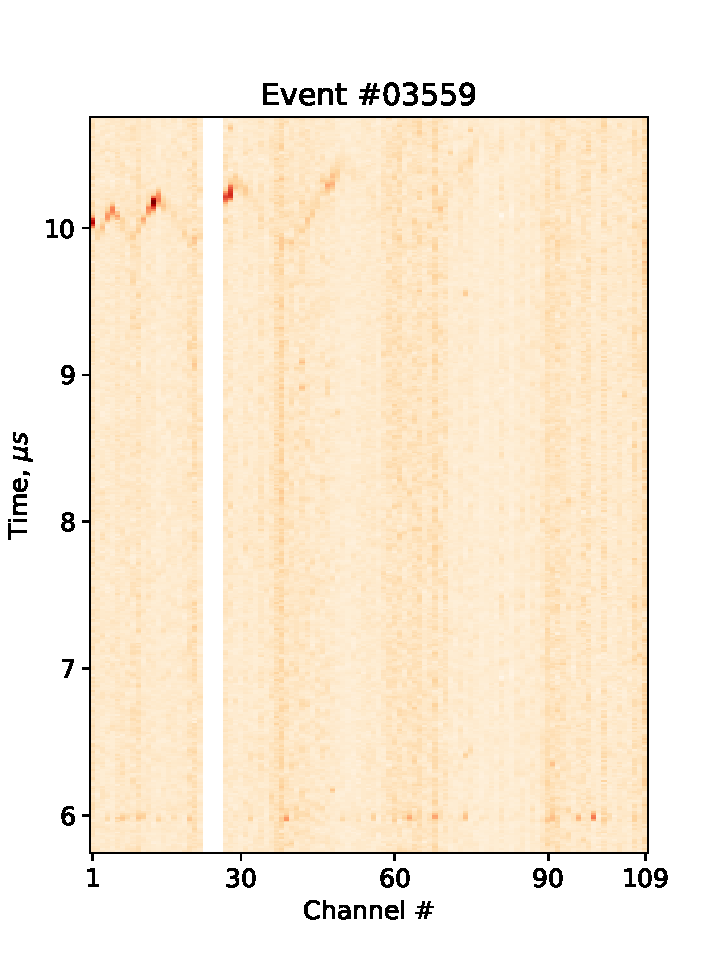
\includegraphics[width=\textwidth]{hybrid-event-1}
            \caption{Direct and reflected CL}
            \label{fig:hybrid-1}
        \end{subfigure}
        \caption{EAS Cherenkov light as seen by the SPHERE-2 detector. The `waves' on the images correspond to the reflected CL (a). The `line' at 6~$\mu$s mark on panel (b) is a direct CL that penetrated the detector enclosure. %\todoi{Нужна ссылка на расшифровку змейки здесь и в тексте.} % нет, не нужна, кто хочет - сам читает материалы СФЕРЫ-2
        }
        \label{fig:foobar}
    \end{minipage}
\end{figure}

%The detector optical scheme is fixed in angular terms which means that each sensitive element receives a certain area on the ground --- its field of view (FOV). This area (FOV) is not static and depends on momentary position and orientation of the detector. An analogy can be drawn with a ground EAS arrays like, for example, the Tunka experiment~\cite{Berezhnev2012}. In the ground-based array each single detector station is analogous to our sensitive element's FOV. And the entire array is analogous to entire FOV of our detector. The main difference between the two cases is the size of the detectors/FOV relative to the distance between them. The SPHERE detectors' sensitive element's FOV is typically 30--100~m in diameter depending on detector altitude, which is greater than the distance between the centers of two adjacent elements FOVs and, in fact, adjacent FOVs overlap. This means that each point on the observation level within the detector's overall FOV does contribute to at least one such integral. This allows the SPHERE detector to observe the near-axis region of the EAS which presents opportunity for improved precision of CL lateral distribution reconstruction \cite{chu74:VKKL74, Anokhina2009}.

The detector optical scheme is designed so that each point of the observation plane within certain area (detector's field of view) is observed by at least one sensitive element of the detector. This allows the SPHERE detector to observe the near-axis region of the EAS which presents opportunity for improved precision of CL lateral distribution reconstruction \cite{chu74:VKKL74, Anokhina2009}.

% PCA!!!! нам надо подумать про PCA подход к поиску критерия. Это упростит нам жизнь.

\subsection{Direct Cherenkov light}

In addition to the main registration method --- the reflected EAS CL --- the SPHERE detector can observe direct CL hitting it from above. EASs with a small zenith angles can be observed both directly and after reflection. Such hybrid events, albeit rare, can be considered the gold standard, providing cross-validation of the reconstruction of arrival angle and CL LDF normalization. 

% A single data point with relatively low angular distribution does not provide much data on primary particle energy and type on its own. But since the direct CL will be registered by the same sensitive element within same `frame' the precision of time measurements is expected be up to 3--5 ns. This timing information will significantly increase the precision of the primary particle arrival direction since the delay between the arrivals of the direct and reflected CL strongly depend on the EAS zenith angle. The measured total flux of the direct CL can also provide constrains on the primary particle energy and axis location. In combination with CL LDF reconstructed from the reflected CL the direct CL form data for the primary particle mass estimation hybrid criteria.

%The idea of the direct CL registration came about by accident. 
The SPHERE-2 detector data contained events in which a rather strong signal was registered by several PMTs simultaneously. The time structure of these events suggested that no reflected light flash could produce them due to significant arrival delays between different PMTs. These events, however, could be explained by direct CL hitting the PMT mosaic from above after penetrating through detector cover and slits in the mirror. Moreover, for some direct CL events a signal from the reflected CL was observed after a time delay corresponding to the EAS light `detector-surface' round trip. An example is shown in Fig.~\ref{fig:foobar}.

%\begin{figure}
%    \centering
%    \begin{subfigure}[b]{0.45\textwidth}
%        \centering
%        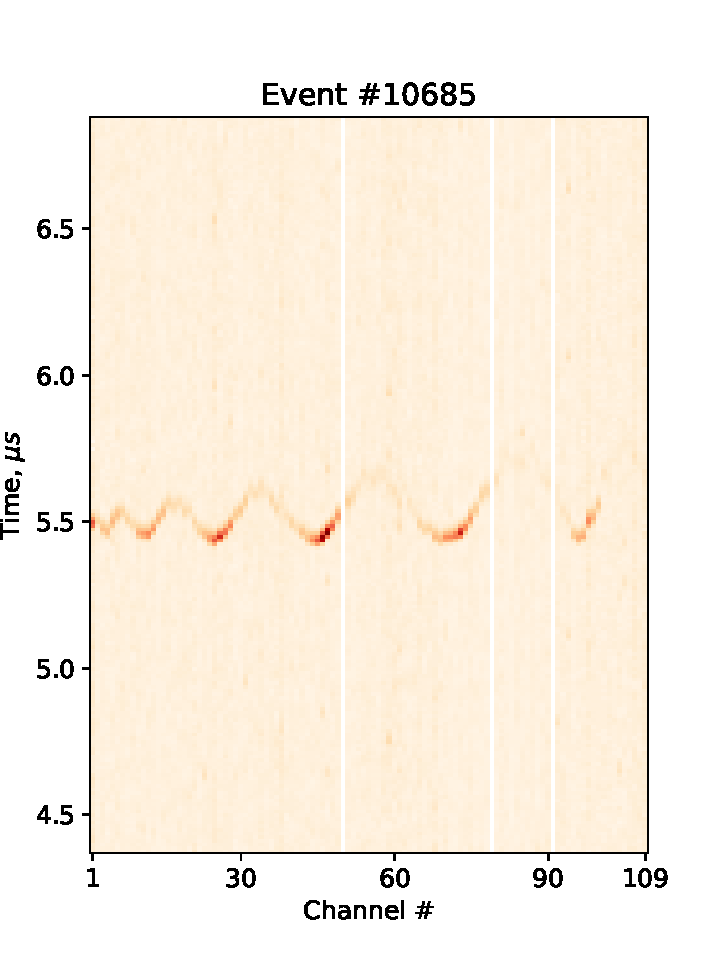
\includegraphics[width=\textwidth]{reflected-event}
%        \caption{Reflected CL event}
%        \label{fig:reflected-ev-1}
%    \end{subfigure}
%    \begin{subfigure}[b]{0.45\textwidth}
%        \centering
%        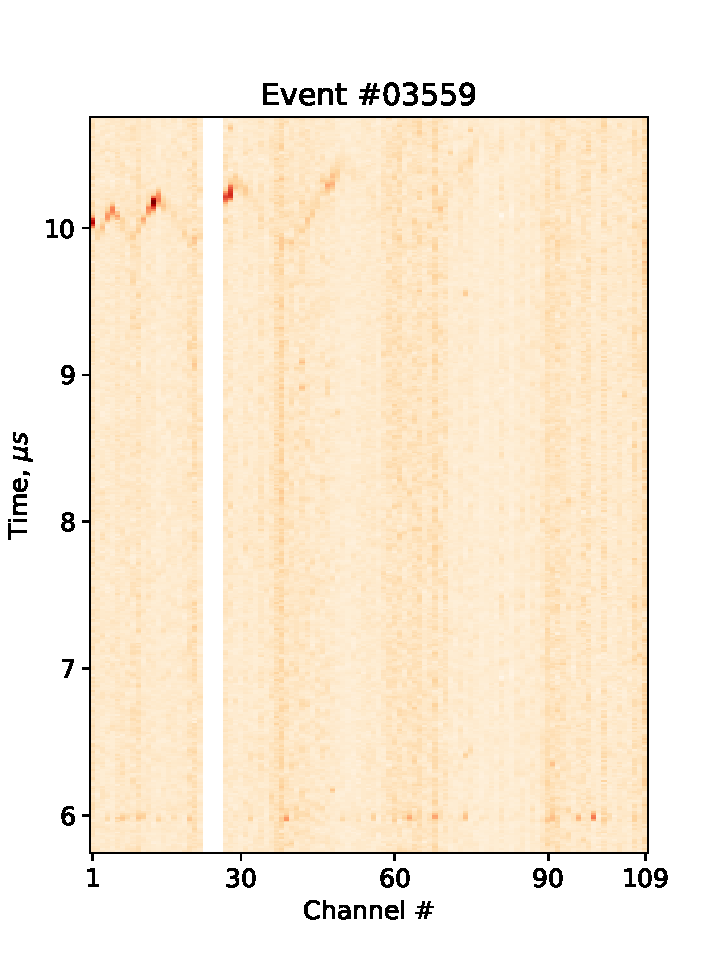
\includegraphics[width=\textwidth]{hybrid-event-1}
%        \caption{Direct and reflected CL (hybrid event)}
%        \label{fig:hybrid-1}
%    \end{subfigure}
%    \caption{EAS Cherenkov light as seen by the SPHERE-2 detector. Сharacteristic wave-like shape of the image is the result of a special spiral channel numbering scheme and serves presentation purposes only. The 'waves' on the images correspond to the reflected CL from the EAS front. The 'line' at the bottom of the image (b) is a direct CL that penetrated the detector enclosure. The time delay between the direct and reflected CL signals is in agreement with the `detector-surface' round trip at the shower's zenith angle.}
%    \label{fig:foobar}
%\end{figure}

%The SPHERE-2 detector was designed to be opaque from the top to reduce background light contamination. Moreover, it was almost always shadowed by the air balloon from above, and the few direct CL events were registered with highly inclined detector coming out of this shadow. In the proposed drone-borne installation, however, the top of the detector is directly exposed to CL and can be intentionally designed to observe it.

The SPEHRE-2 detector was designed with to be shielded from direct CL to reduce background. However, the central part of the detector mirror is almost always shadowed by the sensitive camera from below and does not participate light collection. Therefore, it can can be used as a coded aperture for the direct CL. The accurate selection of the aperture will allow reconstruction of the CL arrival direction (that is different from EAS arrival direction). In specific cases (near detector shower axis location) the angular distribution of the CL at detector level should also be accessible. The additional modeling and analysis is required to correctly estimate impact of this data on overall detector performance.

%It should be noted, however, that the idea of the direct CL registration and the possibility of using hybrid events for cross-validation and calibration of the detector is still speculative and more detailed investigation is underway.

\section{The SPHERE-3 detector}

The proposed SPHERE-3 detector is a logical development of previous SPHERE project implementations. A detailed technical description of the most recent of them, SPHERE-2, can be found in~\cite{Antonov2020}.

\begin{figure}
        \centering 
        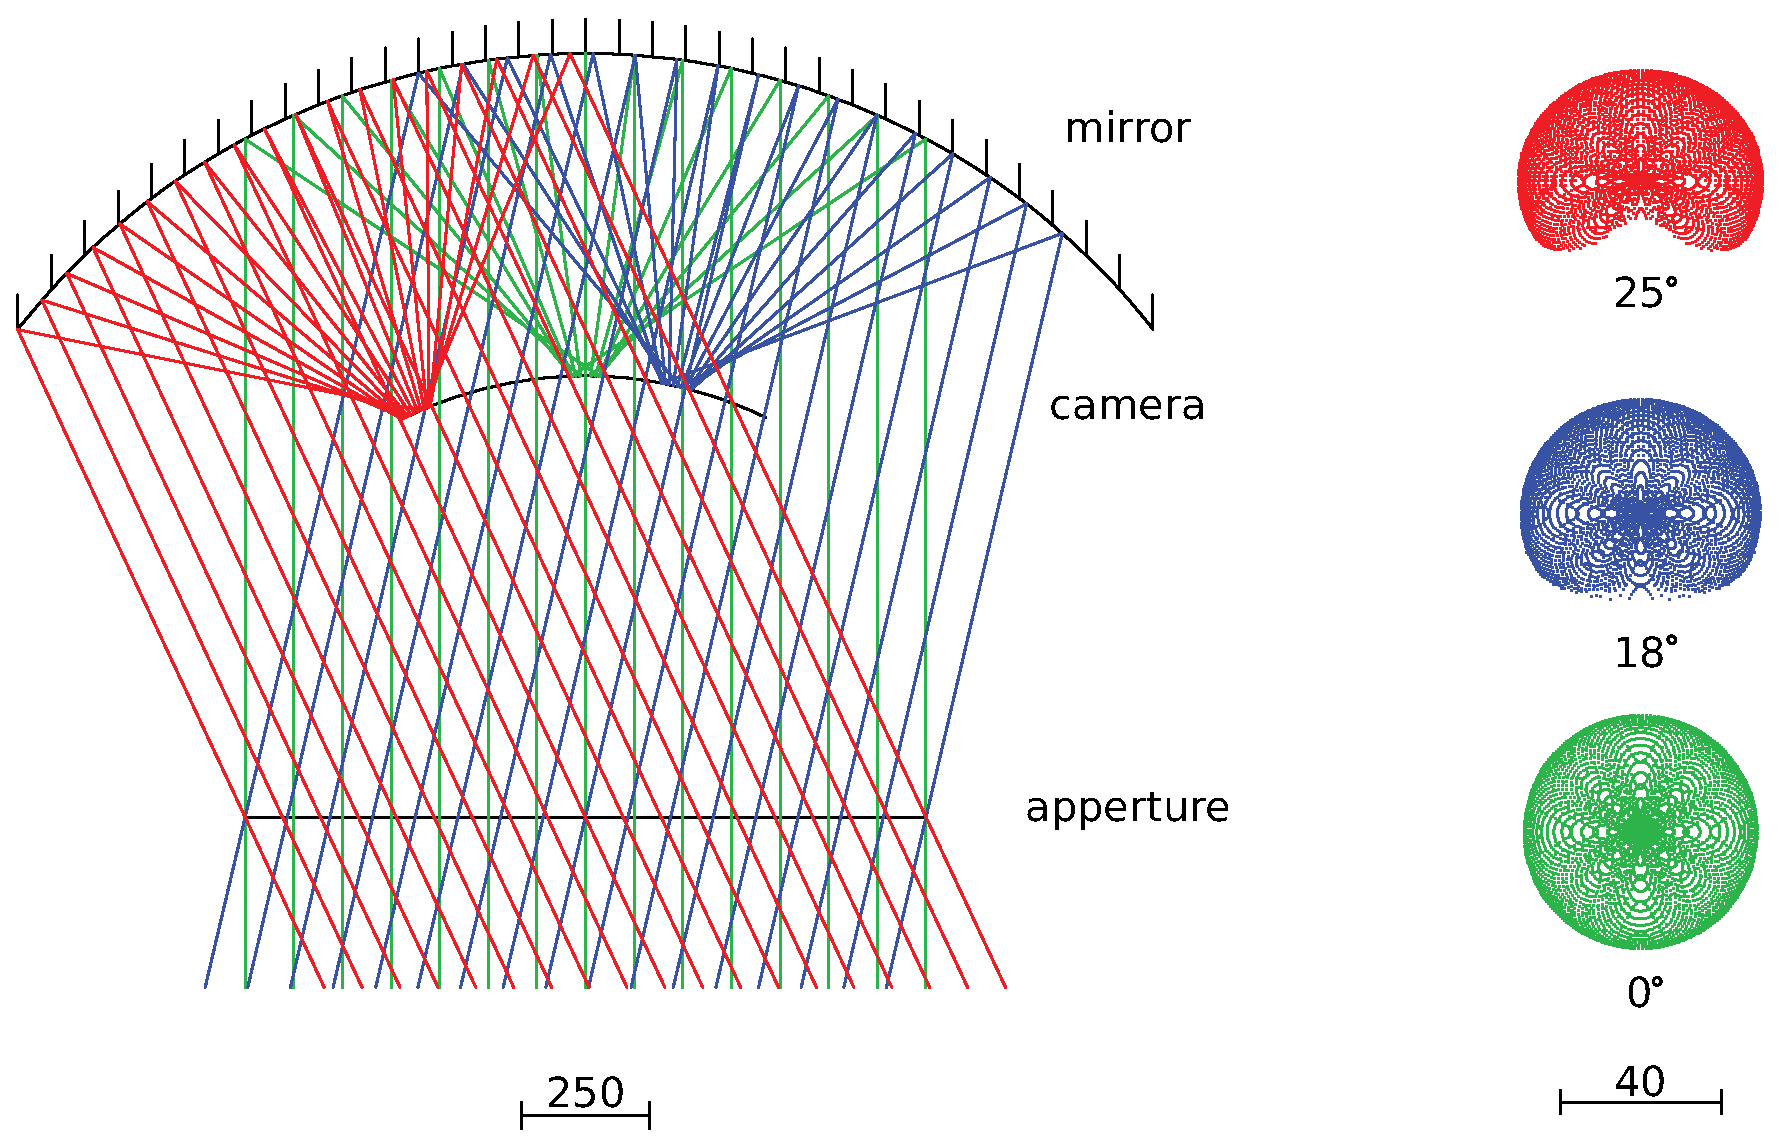
\includegraphics[height=.35\textheight, angle=0]{Sphere3optic_combo.eps}
        \caption{Optical system of the SPHERE-3 detector (on the left). The straight horizontal line represents the aperture limiting incoming light angles; the small curve inside the mirror represents sensitive elements mosaic. Corresponding spot diagram analysis for each direction is presented on the right. Note that the spots take the shadow from the mosaic into account.}
        \label{fig:optical-system}
\end{figure}

%\subsection{Detector design}

Previous SPHERE project implementations detectors with photomultiplier tubes used as sensitive elements were lifted by a balloon to an altitude of 400--900~m~\cite{Ant15a}. The new detector is designed with silicon photomultipliers (SiPM) as sensitive elements to be lifted on a drone (unmanned aerial vehicle, UAV). 

The new detector is a simplified Schmidt scheme telescope without a corrector plate. This mechanically simple and lightweight design is illustrated on Figure~\ref{fig:optical-system}. The uncorrected spherical aberrations serve a purpose of light spot enlargement to be about the size of a sensitive element (SiMPs with light collectors). The light spots size can also be fine-tuned to desired diameter by shifting the mosaic slightly off-focus. This well-established design was used in previous SPHERE implementations and proved itself to be reliable.

For our proposed direct CL observation technique we consider the basic coded aperture in the form of a pattern of 1~cm$^2$ holes. This will allow reconstruction of the direct CL arrival direction (different from EAS arrival direction) and in some cases its angular distribution. Other options may be explored for higher sensitivity or better angular resolution.

The exact technical details of the proposed detector design are not settled because they depend largely on the design and effective payload weight of the carrier drone. We consider a small-aperture ($0.1$~m$^2$) prototype detector, light enough to be lifted by many available heavy lift drones. The target detector is much larger, with up to $1$~m$^2$ aperture and a weight at the upper limit of the payload mass even for the heaviest agriculture drones. Approximate parameters for these two implementations are listed in Table~\ref{tab:detector-specs}.

%\todoi{надо как-то где-то GPS помянуть, не?}

Based of the known parameters and performance of the SPHERE-2 detector for the new detector registration threshold can be estimated to be 3--5~PeV for primary protons with 15$^\circ$ zenith angle in Baikal winter conditions at 700~m flight altitude. 1~PeV threshold can be achieved with lower altitude.

Successful construction of the detector allows for direct experiment scaling by simultaneous operation of several detectors. This will proportionally increase the detector's effective area and statistics.

\begin{table}[t]
\centering
    \caption{Proposed characteristics of the detector and small scale prototype.}
    \label{tab:detector-specs}
    \begin{tabular}{ l c c}
        \toprule
        \textbf{Parameter}  & \parbox[t][.8cm]{3cm}{\centering{\textbf{Prototype of\\the detector}}} & \parbox[t][.8cm]{2cm}{\centering{\textbf{Target\\Detector}}} \\ [1.5ex]
        \midrule
        Effective aperture, m$^2$   & 0.1 & 1.0\\ 
        Mirror diameter, mm         & 800 & 2200\\
        Mirror curvature radius, mm & 500 & 1400\\
        Diaphragm diameter, mm      & 460 & 1320\\
        Sensitive camera diameter, mm&260 & 700\\
        Sensitive camera diameter curvature radius, mm & 300 & 800\\
        Aperture mirror distance on axis, mm & 775 & 1480\\
        Viewing angle of the optical system & \multicolumn{2}{c}{$\pm$25$^\circ$} \\
        Number of pixels & 133 &  up to 1000* \\
        Maximum detector weight, kg &  10  & 100  \\
        Maximum flight altitude, m &  500 & 2000 \\
        \bottomrule
    \end{tabular}
    
\vspace{1mm}
\footnotesize \raggedright 
\hspace{5mm}* Not yet finalized.
\normalsize

\end{table}

%\subsection{Calibration}

Additional registration by the detector of a bright artificial flash with a known brightness distribution across the surface can serve for general experiment calibration that includes snow surface geometrical profile and reflective properties, atmospheric transparency, detector elements sensitivity. With information on the exact SiPM sensitivity from local calibration further analysis of the surface properties can be performed forming independent `image' of the surface that will reduce influence of flashes brightness fluctuations and corresponding uncertainties.

%\subsection{Carrier drone}

The main drone carrying the detector is a key part in a successful operation of the experiment. The main requirements for the drone are a high payload weight and at least 1 hour flight time at the required altitude. The most heavy lifting drones on the market are agricultural drones used for crops spraying (for example, Braeron ИД-400А). Those are gasoline-powered several meters in size multi-engine copters with and up to $200$~kg payload. However, many series of smaller drones are already available and can be used to carry small detector prototype.

Experiment scaling can be achieved with simultaneous operation of several such drones with similar detectors.The drone swarm technique allows multiple drones to interact with each other to avoid mid-air collisions. This is not achievable with a balloons used in previous SPHERE implementations.

%\subsection{Auxiliary drone}

Besides the carrier drone with the detector we plan to use an auxiliary drone to control the atmosphere and snow condition and perform detector calibration. The atmosphere monitoring includes pressure, temperature and humidity continuous measurements up to several kilometers altitude. From that the lower atmosphere profile and it's transparency for CL can be reconstructed and used in modelling and analysis. 

Auxiliary drone can be used for detector calibration as we plan to install on it bright UV and visible light LEDs that will produce direct and reflected light pulses. Concrete applications of the auxiliary drone are covered in Section~\ref{sec:measurement-conditions}.

\section{Measurements conditions}
\label{sec:measurement-conditions}

%\subsection{Atmosphere properties}

Estimation of atmospheric conditions, namely density profile, is crucial for EAS experiments, and especially for CL modelling~\cite{Bernlhr2000}. Even without the auxiliary drone some information about the lower atmosphere can be retrieved from pressure and temperature measured on the detector itself. In the SPHERE-2 experiment pressure and temperature data from the detector along with ground-level measurements was used to choose possible atmosphere density profiles from the set of standard profiles provided by CORSIKA. Even though the flight altitude of the SPHERE-2 was not sufficient to fully characterise even the lowest part of the atmosphere it was sufficient to exclude some models contradicting our data. This very basic assessment allowed to significantly lower the uncertainty coming from the atmosphere model selection.% to around 5--10\% near the axis and less than 5\% in the outer region ($R \gtrapprox 200$~m). The usage of auxiliary drone is expected to reduce this uncertainty down to a few percent. 
 The SPHERE-2 data showed that the atmospheric density profile is quite dynamic and varying significantly between observation nights. Moreover, known weather synopsis along with pressure and temperature on the observation level does not give enough information to correctly estimate factual atmosphere density profile. %But an auxiliary drone will allow continuous monitoring of the atmosphere and later account for it's changes in modelling and events analysis.

%\subsection{Surface properties}

%As mentioned above, bright light flash with known distribution across the surface will give enough data to estimate the surface local reflective properties. With both the detector and flash origin positions known the surface shape can be reconstructed from the timing data of light arrival to the detector. 

%The exact shape of the observation level is important for both the correct estimation of the shower arrival direction (analogous to the exact 3D-positioning of ground based arrays stations) and for the estimation of the CL photons density.

\section{Analysis methods}

The SPHERE project is aimed at further development of reflected EAS CL technique CR studies. This requires not only new technical solutions but also some original analysis methods. We highlight our latest developments in this area with remarks on how these affect the design of the proposed detector.

%\subsection{CL distribution reconstruction}

The SPHERE experiment in its events analysis relies on the EAS CL photons distribution. However, since the detector observes a relatively large area with each sensitive element specific analysis approaches were required and were developed for the SPHERE-2 detector. Moreover, the compact detector design allowed to use topological trigger and full recording of signals from each sensitive element, not only from ones that met trigger condition. These `weak' sensitive elements do contain pulses from EAS CL but of low amplitude on the level on background fluctuations. For example in Fig.~\ref{fig:foobar}(a) channels around 60 contain signals below trigger threshold. 

Since the detector is small the actual number of EAS CL photons reaching its sensitive elements is also small (10--1000 photons per pixel). With significant area observed by each element the collection time due to geometrical effects is also relatively large (up to 150~ns). All this makes each light pulse to be comparable to the background illumination fluctuations. 

%The first challenge in SPHERE data processing is estimating Cherenkov light distribution on the ground. Whereas ground array experiment has direct access to it, measuring light fluxes at scattered points, the SPHERE detector collects light from relatively large area per sensitive element. Moreover, the collected light (both background and EAS Cherenkov light) has a significantly reduced intensity (a coefficient of the order of $10^{-6}$ for a detector lifted to $600$~m), which increases the role of fluctuations and demands special care to be taken when separating EAS signal from background fluctuations.

%Another feature of the SPHERE detector is compact arrangement of all the electronics, allowing for centralized trigger processing. Thanks to this, each experimental event includes channels with signals below trigger level that would not be recorded in a sparse ground array with per-station triggers. Some of these channels include weak signals that can be used in analysis. The processing of these signals also requires special care to be taken during signal-noise separation.

%The first problem is solved by a detailed optical model of the detector, with account of its exact position and orientation at a given time, and use of that model to calculate FOVs for each sensitive element. Each FOV is characterised by the light collection efficiency as a function of observation plane coordinates, that is, a dimensionless function $f(x, y)$ such that for the downward light flux density $Q(x, y)$ the light intensity received by the sensitive element is given by $\int_{\infty} Q(x, y) f(x, y)\,dx\,dy$. Thus, $f(x, y)$ fully determines the relation between ground-level CL distribution and observed photon counts. The set of $f_i(x, y)$ for all sensitive elements is calculated on the event-by-event basis.

%With the SPHERE-3 optical scheme being very close to the previous implementations, this method is also applicable to the proposed detector. The main difference is greater number of sensitive elements, which leads to increased precision in CL distribution reconstruction, especially in near-axis region.

%Another challenge is due to a relatively non-standard use of SiPMs or PMTs for low intensity flashes registration. 
Additionally, registration of low intensity light pulses with PMTs or SiPMs has the inherent randomness of the physical processes behind multiplication that play crucial role in output signal formation. %The common PMTs of SiPMs applications either go for photons counting modes, where only a fact of photoelectron generation is registered, but not the amplitude of resulting pulse, or for large number of photons registration, both in bright flashes or in low fluxes with long exposures, where large numbers even out random effects to their average values. In the case of low intensity short pulses, e.g. low numbers of photons arriving in peak resolution time, the multiplication factor of the PMT or SiPM should be treated as a random variable with specific distribution function.

For photon counts estimation from a recorded anode current impulse we developed a method of statistical deconvolution that allows input information recovery of the linear system with some random qualities from its output treated as a single realization of a random process. After deconvolution, which yields estimation of overall photon count in each time bin, the EAS signal can be separated from the background photons.

For the proposed detector the situation is expected to be slightly different as SiPMs have different multiplication distribution (narrow peak with width significantly lower than its mean); cross-talk between micro-cells of the SiPM; significantly different form of the current pulse on a fast output form a single photoelectron with strong negative afterpulse; significanly higher overall amplification. All this is expected to affect reconstruction in a favorable way in the end, however the results do depend on electronics performance that is not yet finalised.

%\todoi{Дописать про ожидаемые отличия SiPM: больший коэффициент усиления -> меньше погрешность округления, что ещё??}

%\subsection{Shower parameters estimation}

After the reconstruction of the CL photons distribution all relevant shower parameters can be estimated. This can be done by various methods, generally relying on Bayesian statistics framework.

The primary particle arrival direction coincides with the shower axis orientation and is routinely estimated using the relative signal times in several sensitive elements of the detector with respect to detector geometry. Another possibility, unique for the SPHERE detector, is that the temporal signal structure in a given sensitive element depends on its orientation relative to the shower arrival direction. Thus, it carries additional information about the shower's arrival direction and can be used to improve the accuracy of the procedure \cite{Antonov2020}.

%The axis position can be estimated on its own as a point on the ground, from which the LDF decreases monotonously with distance from shower axis. This is a rather simplistic approach, but independent from the assumptions about the LDF shape. A more sophisticated approach may include the axis position as a parameter into the overall LDF shape fitting procedure.

Finally, primary particle energy can be estimated from the CL LDF with numerous methods, generally relying on the fact that overall number of Cherenkov photons is approximately proportional to the primary energy. Some of the methods involve analytical LDF approximations \cite[e.g.][]{AlRubaiee2014}, others rely on direct comparison between Monte-Carlo-modelled LDF with an observed values~\cite{Antonov2015}.

%\subsection{Primary type}
%\todoi{кажется это надо сокращать вплоть до слов "по наклону ФПР, см. поодробности по ссылкам"}
%Modeling procedure generally follows the approach used in SPHERE-2 experiment. It includes event modeling and image processing.
%Event modeling incorporates two stages: a) EAS simulation with CORSIKA code including Cherenkov light generation and b) the production of CL images of EAS events in the telescope mosaic. The 1st stage results in a detailed 3D-array of CL photoelecton distribution in coordinates and time delay on the snow for each EAS event. Photoelectons appear due to a special CORSIKA mode enabling account for the PMT efficiency during the shower modeling. At the 2nd stage the shower cores on the snow are evenly spread over a circle of 500 m radius centered under the telescope. Contributions to the mosaic PMTs from every patch of the CL spot on the snow are calculated on photoelectron-by-photoelectron basis.

The primary mass estimation is a remarkably hard problem and no generally agreed upon method is known at the time. Moreover, different experiments report conflicting CR mass compositions in PeV--EeV energy ranges. This makes the problem especially interesting, given the promise of the SPHERE project to refine existing methods using information about near-axis structure of CL LDF.

The main idea of the mass estimation procedure follows previous works, e.g. using the LDF shape \cite{Anokhina2009} via area integrals optimized to certain zenith angles and energies. %In the SPHERE project the shower mass-sensitive parameter is a CL LDF slope and usually constructed as a ratio of two integrals:
%\begin{equation}
%$    \eta = {\int\limits_{r_1}^{r_2}Q(r)r\,dr} \Big / {\int\limits_{r_3}^{r_4}Q(r)r\,dr}
%$
%\end{equation}
%\marginpar{Не, тут от r1 до r2 и от r3 до r4, а вот то, что r1=0 и r3=2 - это уже конктретный подбор для вертикальных ливней 10 ПэВ}
%Such parameter can be optimized with regard to the shower primary energy, zenith arrival angle, detector altitude and atmosphere model. This is done by varying inner and outer integration radii $r_1, ..., r_4$ to achieve the best possible degree of separation between different primary mass-groups. The exact criteria values for this parameter also depend on the number of mass-groups.
Another possibility to improve the primary mass resolution is the use of the direct CL angular distribution which is proved to be a powerful instrument for this task~\cite{Gal18a}.

Besides optimizing mass-estimation procedure for a given detector altitude and construction, we can do the opposite. With most detector parameters still not fully determined we plan to evaluate the mass separation criteria as a function of detector parameters and choose the best configuration for this task.

\section{Summary}
A new detector SPHERE-3 is being developed in the SPHERE project for cosmic ray studies using reflected EAS CL method. SPHERE-3 is expected to be a technical upgrade over SPHERE-2 detector in regards to the electronics and sensitive camera. A switch in carrier from a balloon to the drone should simplify running and reduce cost that in perspective will horizontal scaling of the experiment. 

Upgrade from PMTs to SiPMs will increase effective sensitivity of the detector that will allow smaller pixels and in turn better spacial resolution that will greatly increase sensitivity to the primary particle type.

Addition of the auxiliary drone atmosphere parameters monitoring and detector calibration should help to reduce systematic experimental uncertainties.

\acknowledgments
M. Finger and M. Finger Jr thank MEYS of Czech Republic for grants LG14004 and LG18022.

\bibliographystyle{JHEP}
\bibliography{references}

\end{document}
